% Pagina originale 36
\pagina{36}
\section*{Quadratura}
La quadratura è una tecnica che consente di calcolare
\[\int_a^b f(x)\,dx=I(f)\]
conoscendo $f(x)$ nell'intervallo $[a,b]$, quando diventa difficile o costoso calcolare $F(x)$ o quando si conoscono solo un certo numero di punti appartenenti ad $f(x)$.
\subsection*{Formule di quadratura di tipo interpolatorio}
\[\sum_{k=0}^m w_k f(x_k)\simeq I(f).\]
Formule di quadratura con $x_k$ nodi e $w_k$ pesi. Poniamo $f(x)=L_m(x)+e(x)$:
\begin{align*}
\int_a^b f(x)\,dx&=\int_a^b L_m(x)\,dx+\int_a^b e(x)\,dx\\
&=\int_a^b\sum_{k=0}^m\ell_{mk}(x)f(x_k)\,dx+\int_a^b e(x)\,dx\\
&=\sum_{k=0}^m\left[\int_a^b\ell_{mk}(x)\,dx\right]f(x_k)+\int_a^b e(x)\,dx.
\end{align*}
Pongo
\[w_k=\int_a^b\ell_{mk}(x)\,dx,\qquad R_{m+1}(f)=\int_a^b e(x)\,dx.\]
Le $\ell_{mk}$ sono le formule interpolatrici; $R_{m+1}(f)$ è il resto della formula di quadratura:
\[\boxed{I(f)=\sum_{k=0}^m w_k f(x_k)+R_{m+1}(f)},\qquad I(f)\simeq\sum_{k=0}^m w_k f(x_k).\]
\subsection*{Grado di precisione}
Una formula ha grado di precisione $q$ se fornisce il valore esatto di $I(f)$ quando $f$ è un polinomio di grado al più $q$ e $\exists p(x)\in\mathcal P_{q+1}\setminus\mathcal P_q$ tale che $R_{q+1}(f)\ne0$.
% Pagina originale 37
\pagina{37}
\textbf{Osservazione.} Ogni formula di quadratura di tipo interpolatorio ha grado di precisione $q\ge m$ ($m=\text{numero dei nodi}-1$).
\textbf{Dimostrazione.}
\[\int_a^b p_m(x)\,dx=\sum_{i=0}^m w_i p_m(x_i)+R_{m+1}(f),\]
\[R_{m+1}(f)=\int_a^b e(x)\,dx=\int_a^b\omega_{m+1}(x)\frac{p_m^{(m+1)}(x)}{(m+1)!}\,dx\equiv0,\]
poiché $p_m^{(m+1)}(x)=0$ per ogni $p_m\in\mathcal P_m$.
\subsection*{Formule di Newton--Cotes}
Suddivido $[a,b]$ in $m$ sottointervalli di ampiezza $h$, con
\[h=\frac{b-a}{m},\qquad x_i=a+ih,\quad i=0,1,\ldots,m.\]
\[\int_a^b f(x)\,dx=\sum_{i=0}^m w_i f(x_i)+R_{m+1}(f)\]
è la formula di Newton--Cotes.
\textbf{Proprietà:} $w_i=w_{m-i}$ (proprietà di simmetria).
\textbf{Dimostrazione.}
\[c=\frac{x_i+x_{m-i}}2=\frac{b+a}2\quad\Longrightarrow\quad
\begin{cases}x_i=2c-x_{m-i},\\x_{m-i}=2c-x_i.\end{cases}\]
\begin{align*}
w_k&=\int_a^b\prod_{\substack{i=0\\i\ne k}}^m\frac{x-x_i}{x_k-x_i}\,dx\\
&=\int_a^b\prod_{\substack{i=0\\i\ne k}}^m\frac{x-2c+x_{m-i}}{2c-x_{m-k}-2c+x_{m-i}}\,dx\\
&=\int_a^b\prod_{\substack{i=0\\i\ne k}}^m\frac{2c-x-x_{m-i}}{x_{m-k}-x_{m-i}}\,dx.
\end{align*}
Posto $t=2c-x$, si ha $t=2c-a=b$, $t=2c-b=a$, $dt=-dx$: si scambiano gli estremi di integrazione,
\[\int_a^b f(x)\,dx=-\int_b^a f(t)\,dt=\int_a^b f(t)\,dt.\]
Quindi
\[w_k=\int_a^b\prod_{\substack{i=0\\i\ne k}}^m\frac{t-x_{m-i}}{x_{m-k}-x_{m-i}}\,dt
=\int_a^b\prod_{\substack{j=0\\j\ne m-k}}^m\frac{t-x_j}{x_{m-k}-x_j}\,dt=w_{m-k},\qquad j=m-i.\]
% Pagina originale 38
\pagina{38}
\subsection*{Formula dei trapezi}
\[x_0=a,\quad x_1=b,\quad h=b-a,\qquad T_2=w_0f(x_0)+w_1f(x_1).\]
\begin{center}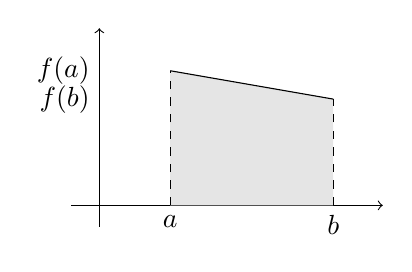
\begin{tikzpicture}[scale=.9]
\draw[->](-.4,0)--(4,0);\draw[->](0,-.3)--(0,2.5);
\fill[gray!20](1,0)--(1,1.9)--(3.3,1.5)--(3.3,0)--cycle;
\draw(1,1.9)--(3.3,1.5);\draw[dashed](1,0)--(1,1.9)(3.3,0)--(3.3,1.5);
\node[below]at(1,0){$a$};\node[below]at(3.3,0){$b$};\node[left]at(0,1.9){$f(a)$};\node[left]at(0,1.5){$f(b)$};
\end{tikzpicture}\end{center}
\begin{align*}
w_0&=\int_a^b\ell_{10}(x)\,dx=\int_a^b\frac{x-x_1}{x_0-x_1}\,dx
=\int_a^b\frac{x-b}{a-b}\,dx\\
&=\frac1{a-b}\left[\frac{(x-b)^2}2\right]_{x=a}^{x=b}
=-\frac{h^2}2\frac1{-h}=\frac h2.
\end{align*}
$a$ e $b$ sono nodi simmetrici rispetto a $c$, quindi $w_0=w_1=h/2$:
\[\boxed{T_2=\frac h2\bigl(f(a)+f(b)\bigr)}\qquad\text{formula dei trapezi}.\]
\subsection*{Resto nella formula dei trapezi}
\[R_2(f)=\frac1{2!}\int_a^b(x-a)(x-b)f''(\xi_x)\,dx.\]
Per manipolare quest'espressione abbiamo bisogno di conoscere il teorema della media generalizzato.
\subsection*{Teorema della media generalizzato}
Siano $f,g:[a,b]\to\mathbb R$, $f$ continua, $g(x)$ a segno costante e $g(x)\ne0$ per ogni $x\in(a,b)$. Allora
\[\int_a^b f(x)g(x)\,dx=f(\bar x)\int_a^b g(x)\,dx,\qquad\bar x\in[a,b].\]
Poiché $(x-a)(x-b)$ è a segno costante,
\[\int_a^b(x-a)(x-b)f''(\xi_x)\,dx=f''(\eta)\int_a^b(x-a)(x-b)\,dx\]
e quindi
\[R_2(f)=\frac{f''(\eta)}{2!}\int_a^b(x-a)(x-b)\,dx.\]
% Pagina originale 39
\pagina{39}
Posto $h=b-a$ e $x=a+ht$, con $t\in[0,1]$, $dx=h\,dt$:
\begin{align*}
R_2(f)&=\frac{f''(\eta)}{2!}\int_0^1 ht(-h+ht)h\,dt\\
&=\frac{f''(\eta)}{2!}\int_0^1 h^3t(t-1)\,dt
=\frac{f''(\eta)}{2!}h^3\left[\frac{t^3}3-\frac{t^2}2\right]_0^1
=-\frac{h^3}{12}f''(\eta).
\end{align*}
$R_2(f)=0\Longleftrightarrow f\in\mathcal P_1$. Il grado di precisione è $q=1$ (con $f$ di grado $2$, $R_2(f)\ne0$).
\subsection*{Formula di Simpson}
\[x_0=a,\quad x_2=b,\quad x_1=c=\frac{b+a}2,\qquad h=\frac{b-a}2,\]
\[S_3=w_0f(a)+w_1f(c)+w_2f(b).\]
\[w_0=\int_a^b\ell_{20}(x)\,dx=\int_a^b\frac{(x-b)(x-c)}{(a-b)(a-c)}\,dx.\]
Posto $x=c+ht$, $dx=h\,dt$:
\begin{align*}
w_0&=\int_{-1}^1\frac{(ht-h)(ht)}{(-2h)(-h)}h\,dt
=\int_{-1}^1\frac{(t-1)ht}2\,dt\\
&=\frac h2\left[\frac{t^3}3-\frac{t^2}2\right]_{-1}^1
=\frac h2\left(-\frac16+\frac56\right)=\frac23\frac h2=\frac h3.
\end{align*}
$w_0=w_2=h/3$ per simmetria.
\begin{align*}
w_1&=\int_a^b\ell_{21}(x)\,dx=\int_a^b\frac{(x-a)(x-b)}{(c-a)(c-b)}\,dx\\
&=\int_{-1}^1\frac{h(1+t)(ht-h)}{h(-h)}h\,dt
=h\int_{-1}^1(1-t^2)\,dt\\
&=h\left[t-\frac{t^3}3\right]_{-1}^1=h\left(\frac23+\frac23\right)=\frac43h.
\end{align*}
% Pagina originale 40
\pagina{40}
\[\boxed{S_3=\frac h3\bigl(f(a)+4f(c)+f(b)\bigr)}\qquad\text{formula di Simpson}.\]
\[\boxed{R_3(f)=-h^5\frac{f^{(4)}(\sigma)}{90}},\quad\sigma\in(a,b),\qquad h=\frac{b-a}2.\]
Grado di precisione $q=3$.
\subsection*{Formula del punto di mezzo}
Sia $c=(a+b)/2$. Sviluppo la serie di Taylor con $c$ punto iniziale:
\[f(x)=f(c)+f'(c)(x-c)+\frac{f''(\xi_x)}{2!}(x-c)^2,\qquad\xi_x\in[a,b].\]
\begin{align*}
\int_a^b f(x)\,dx&=\int_a^b f(c)\,dx+f'(c)\underbrace{\int_a^b(x-c)\,dx}_{0}
+\int_a^b\frac{f''(\xi)}2(x-c)^2\,dx\\
&=f(c)(b-a)+\int_a^b\frac{f''(\xi)}2(x-c)^2\,dx.
\end{align*}
Posto $h=b-a$, $\int_a^b f(x)\,dx\simeq hf(c)$.
\begin{align*}
R(f)&=\int_a^b\frac{f''(\xi)}2(x-c)^2\,dx
=\frac{f''(\eta)}2\int_a^b(x-c)^2\,dx\\
&=\frac{f''(\eta)}2\left.\frac{(x-c)^3}3\right|_a^b
=\frac{f''(\eta)}2\left(\frac{h^3}{24}+\frac{h^3}{24}\right)=\frac{h^3}{24}f''(\eta).
\end{align*}
\[\boxed{R(f)=\frac{h^3}{24}f''(\eta)},\qquad\boxed{M=hf(c)}.\]
Grado di precisione $q=1$. Il grado di precisione di questa tecnica è uguale a quello del trapezio, ma questa formula necessita solo di un punto.
\subsection*{Formule di quadratura composte}
Consiste nel dividere l'intervallo $[a,b]$ in $N$ sottointervalli con ampiezza uguale, aumentando la precisione.
% Pagina originale 41
\pagina{41}
\[\int_a^b f(x)\,dx=\sum_{i=0}^{N-1}\int_{x_i}^{x_{i+1}} f(x)\,dx,\quad x_i=a+ih,\quad h=\frac{b-a}N.\]
\subsection*{Formula dei trapezi composti}
\begin{align*}
\int_a^b f(x)\,dx&=\sum_{i=0}^{N-1}\left[\frac h2\bigl(f(x_i)+f(x_{i+1})\bigr)-\frac1{12}h^3f''(\eta_i)\right]\\
&=\frac h2\sum_{i=0}^{N-1}\bigl(f(x_i)+f(x_{i+1})\bigr)-\frac1{12}h^3\sum_{i=0}^{N-1}f''(\eta_i)\\
&=\frac h2\bigl(f(x_0)+f(x_N)\bigr)+h\sum_{i=1}^{N-1}f(x_i)-\frac{h^3}{12}Nf''(\eta),
\end{align*}
con $\eta_i\in(x_i,x_{i+1})$ e $\eta\in(a,b)$.
\[\boxed{T_c^{(h)}=\frac h2\bigl(f(x_0)+f(x_N)\bigr)+h\sum_{i=1}^{N-1}f(x_i)}.\]
\[R_T=-\frac{h^3}{12}Nf''(\eta)=-\frac{(b-a)^3}{12N^3}Nf''(\eta)
=\boxed{-\frac{(b-a)^3}{12N^2}f''(\eta)}.\]
Teorema della media nel discreto:
\[\sum_{i=1}^N f(x_i)=Nf(\bar x),\quad x_i\in[a,b],\quad\bar x\in(a,b).\]
Sappiamo che
\[|R_T|\le\frac1{12}\frac{(b-a)^3}{N^2}\underbrace{\max_{x\in(a,b)}|f''(x)|}_{M}.\]
\[\varepsilon\ge\frac1{12}\frac{(b-a)^3}{N_\varepsilon^2}M
\quad\Longrightarrow\quad N_\varepsilon\ge\sqrt{\frac{(b-a)^3M}{12\varepsilon}}.\]
Possiamo stabilire in quanti pezzi suddividere $[a,b]$ per ottenere una precisione $\varepsilon\ge|R_T|$.
\subsection*{Formula di Simpson composta}
Suddivido $[a,b]$ in $N$ intervalli, con $N$ pari:
\begin{align*}
\int_a^b f(x)\,dx&=\sum_{i=0}^{N/2-1}\int_{x_{2i}}^{x_{2i+2}}f(x)\,dx\\
&=\sum_{i=0}^{N/2-1}\left[\frac h3\bigl(f(x_{2i})+4f(x_{2i+1})+f(x_{2i+2})\bigr)-\frac{h^5}{90}f^{(4)}(\eta_i)\right].
\end{align*}
% Pagina originale 42
\pagina{42}
\[\int_a^b f(x)\,dx=\frac h3\sum_{i=0}^{N/2-1}\bigl[f(x_{2i})+4f(x_{2i+1})+f(x_{2i+2})\bigr]-\frac{h^5N}{180}f^{(4)}(\eta).\]
\[\boxed{S_c(h)=\frac h3\left[f(x_0)+f(x_N)+2\sum_{i=1}^{N/2-1}f(x_{2i})+4\sum_{i=0}^{N/2-1}f(x_{2i+1})\right]}.\]
\[R_S=-\frac{h^5N}{90}f^{(4)}(\eta)=-\boxed{\frac{(b-a)^5}{180N^4}f^{(4)}(\eta)}.\]
\emph{Nota di trascrizione (pagina 42): il denominatore 90 nella prima espressione di $R_S$ compare così nell'originale, mentre le espressioni adiacenti hanno 180.}
\[|R_S|\le\frac{(b-a)^5}{180N^4}\max_{x\in(a,b)}|f^{(4)}(x)|,\]
\[\varepsilon\ge\frac{(b-a)^5}{180N_\varepsilon^4}M\quad\Longrightarrow\quad
N_\varepsilon\ge\sqrt[4]{\frac{(b-a)^5M}{180\varepsilon}}.\]
\subsection*{Formula del punto di mezzo composta}
\begin{align*}
\int_a^b f(x)\,dx&=\sum_{i=0}^{N/2-1}\int_{x_{2i}}^{x_{2i+2}}f(x)\,dx\\
&=\sum_{i=0}^{N/2+1}2h f(x_{2i+1})+\sum_{i=0}^{N/2-1}\frac{(2h)^3}{24}f''(\eta_i)\\
&=2h\sum_{i=0}^{N/2+1}f(x_{2i+1})+\frac{h^3}{6}Nf''(\eta).
\end{align*}
\[\boxed{M_c(h)=2h\sum_{i=0}^{N/2-1}f(x_{2i+1})},\qquad
\boxed{R_M=\frac{(b-a)^3}{6N^2}f''(\eta)},\qquad N_\varepsilon\ge\sqrt{\frac{(b-a)^3M}{6\varepsilon}}.\]
\emph{Nota di trascrizione (pagina 42): gli indici $N/2+1$ delle due somme intermedie e il coefficiente del resto sono riprodotti come nella fonte; la formula evidenziata ha indice $N/2-1$.}
\section*{Derivazione numerica}
È una tecnica per trovare le derivate di una funzione senza calcolare effettivamente $f^{(m)}(t)$.
Supponiamo che $f\in C^k([a,b])$ con $k$ sufficientemente grande per i nostri scopi e dividiamo $[a,b]$ in
\[a\equiv t_0<t_1<t_2<\cdots<t_{N-1}<t_N\equiv b.\]
% Pagina originale 43
\pagina{43}
Considero tre punti consecutivi $t_{m-1},t_m,t_{m+1}$:
\[t_{m-1}=t_m-h,\qquad t_{m+1}=t_m+h.\]
\begin{align*}
f(t_{m+1})&=f(t_m)+f'(t_m)h+\frac{f''(t_m)}2h^2+\frac{f^{(3)}(t_m)}6h^3+\frac{f^{(4)}(\xi)}{24}h^4,\\
f(t_{m-1})&=f(t_m)-f'(t_m)h+\frac{f''(t_m)}2h^2-\frac{f^{(3)}(t_m)}6h^3+\frac{f^{(4)}(\eta)}{24}h^4.
\end{align*}
\[f(t_{m+1})+f(t_{m-1})=2f(t_m)+f''(t_m)h^2+\frac{h^4}{24}\bigl(f^{(4)}(\xi)+f^{(4)}(\eta)\bigr).\]
\[f(t_{m+1})+f(t_{m-1})\simeq2f(t_m)+f''(t_m)h^2\]
\[\boxed{f''(t_m)\simeq\frac{f(t_{m+1})+f(t_{m-1})-2f(t_m)}{h^2}}.\]
\[\boxed{E(f''(t_m))=-\frac{h^2}{24}\bigl(f^{(4)}(\xi)+f^{(4)}(\eta)\bigr)=-\frac{h^2}{12}f^{(4)}(\chi)},\quad\chi\in[t_{m-1},t_{m+1}].\]
Provo ad approssimare la derivata prima:
\begin{align*}
f(t_{m+1})&=f(t_m)+f'(t_m)h+\frac{f''(t_m)}2h^2+\frac{f^{(3)}(\sigma_1)}6h^3,\\
f(t_{m-1})&=f(t_m)-f'(t_m)h+\frac{f''(t_m)}2h^2-\frac{f^{(3)}(\sigma_2)}6h^3.
\end{align*}
\[f(t_{m+1})-f(t_{m-1})=2f'(t_m)h+\frac{f^{(3)}(\sigma)}3h^3.\]
\[\boxed{f'(t_m)\simeq\frac{f(t_{m+1})-f(t_{m-1})}{2h}}\qquad\text{formula delle differenze centrali}.\]
\[\boxed{E(f'(t_m))=-\frac{f^{(3)}(\delta)}6h^2},\qquad\delta\in[t_{m-1},t_{m+1}].\]
% Pagina originale 44
\pagina{44}
\subsection*{Differenze in avanti}
Sviluppo con Taylor $f(t_{m+1})$:
\[f(t_{m+1})=f(t_m)+hf'(t_m)+h^2\frac{f''(\sigma)}2\]
\[\boxed{f'(t_m)\simeq\frac{f(t_{m+1})-f(t_m)}h},\qquad
\boxed{E(f'(t_m))=-\frac h2 f''(\sigma)},\quad\sigma\in[t_m,t_{m+1}].\]
\subsection*{Differenze all'indietro}
Sviluppo con Taylor $f(t_{m-1})$:
\[f(t_{m-1})=f(t_m)-hf'(t_m)+h^2\frac{f''(\sigma)}2\]
\[\boxed{f'(t_m)\simeq\frac{f(t_m)-f(t_{m-1})}h},\qquad
\boxed{E(f'(t_m))=\frac h2 f''(\sigma)},\quad\sigma\in[t_{m-1},t_m].\]
\textbf{Nota.} Queste formule hanno ordine $1$ ($E\propto h$), mentre la formula delle differenze centrali ha ordine $2$ ($E\propto h^2$), quindi è più accurata.
\section*{Equazioni differenziali}
Definiamo un problema di Cauchy ai valori iniziali:
\[\begin{cases}y'(t)=f(t,y(t)),\\y(t_0)=y_0,\end{cases}\]
dove $f:[t_0,T]\times\mathbb R\to\mathbb R$, con $f\in C([t_0,T])$ e lipschitziana.
\textbf{Lipschitzianità.} $f$ è lipschitziana rispetto a $y$ se
\[\exists L>0:\quad\forall x,y\in\mathbb R:\quad|f(t,x)-f(t,y)|\le L|x-y|,\qquad\forall t\in[t_0,T].\]
% Pagina originale 45
\pagina{45}
$y(t)$ è soluzione dell'equazione differenziale se rispetta le condizioni del sistema ed è $y\in C^1([t_0,T])$.
Si discretizza l'intervallo di integrazione $[t_0,T]$:
\[t_{m+1}=t_m+h,\qquad t_m=t_0+mh,\quad m=0,1,\ldots,N,\qquad h=\frac{T-t_0}N.\]
\begin{align*}
y'(t)&=f(t,y(t))\\
\Longrightarrow\quad\int_{t_m}^{t_{m+1}}y'(t)\,dt&=\int_{t_m}^{t_{m+1}}f(t,y(t))\,dt\\
\Longrightarrow\quad y(t_{m+1})-y(t_m)&=\int_{t_m}^{t_{m+1}}f(t,y(t))\,dt.
\end{align*}
\subsection*{Metodo di Euler esplicito}
\[y(t_{m+1})-y(t_m)=hf(t_m,y(t_m))+\text{errore}\]
\[y(t_{m+1})-y(t_m)\simeq hf(t_m,y(t_m)).\]
Approssimo $y_{m+1}\simeq y(t_{m+1})$, $y_m\simeq y(t_m)$:
\[y_{m+1}-y_m=hf(t_m,y_m)\quad\Longleftrightarrow\quad
\boxed{y_{m+1}=y_m+hf(t_m,y_m)}.\]
È chiamato metodo di Euler esplicito in quanto, noto $y_m$, è possibile calcolare esplicitamente $y_{m+1}$.
\subsection*{Metodo di Euler implicito}
\[y(t_{m+1})-y(t_m)=hf(t_{m+1},y(t_{m+1}))+\text{errore}\]
\[y(t_{m+1})-y(t_m)\simeq hf(t_{m+1},y(t_{m+1}))\]
\[y_{m+1}-y_m\simeq hf(t_{m+1},y_{m+1})\quad\Longleftrightarrow\quad
\boxed{y_{m+1}=y_m+hf(t_{m+1},y_{m+1})}.\]
% Pagina originale 46
\pagina{46}\subsection*{Metodo dei trapezi}
\[y(t_{m+1})-y(t_m)\simeq\frac h2[f(t_m,y(t_m))+f(t_{m+1},y(t_{m+1}))].\]
\[\boxed{y_{m+1}=y_m+\frac h2[f(t_m,y_m)+f(t_{m+1},y_{m+1})]}.\]
\subsection*{Metodo del midpoint}
\[y(t_{m+2})-y(t_m)\simeq2hf(t_{m+1},y(t_{m+1})),\quad\boxed{y_{m+2}=y_m+2hf(t_{m+1},y_{m+1})}.\]
\begin{center}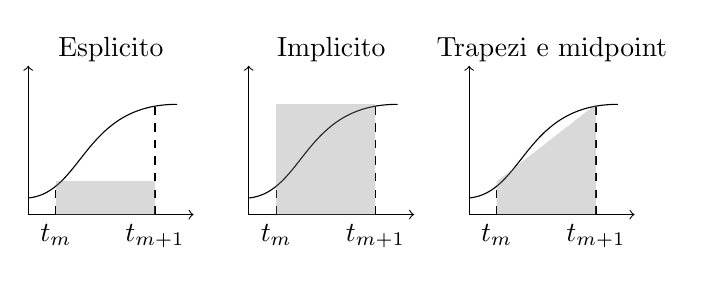
\begin{tikzpicture}[scale=.7]\foreach \d/\lab in {0/Esplicito,4/Implicito,8/Trapezi e midpoint}{\begin{scope}[xshift=\d cm]\draw[->](0,0)--(3,0);\draw[->](0,0)--(0,2.7);\draw(0,.3)..controls(1,.4)and(1,2)..(2.7,2);\draw[dashed](.5,0)node[below]{$t_m$}--(.5,.6)(2.3,0)node[below]{$t_{m+1}$}--(2.3,2);\node at(1.5,3){\lab};\end{scope}}\fill[gray,opacity=.3](.5,0)rectangle(2.3,.6);\fill[gray,opacity=.3](4.5,0)rectangle(6.3,2);\fill[gray,opacity=.3](8.5,0)--(8.5,.6)--(10.3,2)--(10.3,0)--cycle;\end{tikzpicture}\end{center}
\subsection*{Classificazione dei metodi numerici}
Se la soluzione nell'istante $t_{m+k}$ dipende da $k$ valori ottenuti in precedenza $t_{m+k-1},\ldots,t_{m+1},t_m$, il metodo si dice a $k$ passi ($k$-steps). Euler e trapezi sono a un passo (one-step); midpoint è a due passi.
\[y_{m+k}=y_m+h\Phi(t_m,\ldots,t_{m+k},y_m,\ldots,y_{m+k}),\]
\[y_{m+1}=y_m+h\Phi(t_m,t_{m+1},y_m,y_{m+1}).\]
Se $y_{m+1}=y_m+h\Phi(t_m,t_{m+1},y_m)$, o più in generale
\[y_{m+k}=y_m+h\Phi(t_m,\ldots,t_{m+k},y_m,\ldots,y_{m+k-1}),\]
il metodo è esplicito (Euler esplicito e midpoint).
% Pagina originale 47
\pagina{47}
Se ciò non fosse, il metodo è implicito (Euler implicito e trapezi). Per calcolare $y_{m+k}$ in un metodo implicito dovremo risolvere un'equazione che potrebbe non essere lineare se $f(t,y)$ non è lineare.
\[y_{m+1}=y_m+hf(t_{m+1},y_{m+1}),\qquad g(x)=y_m+hf(t_{m+1},x).\]
\[\boxed{y_{m+1}^{(r+1)}=g(y_{m+1}^{(r)})=y_m+hf(t_{m+1},y_{m+1}^{(r)})},\quad y_{m+1}^{(0)}=y_m.\]
Affinché il metodo converga $|g'(x)|<1$:
\[g'(x)=h\frac{\partial f}{\partial y}(t_{m+1},x),\quad\left|h\frac{\partial f}{\partial y}(t_{m+1},x)\right|<1\Longrightarrow h\left|\frac{\partial f}{\partial y}\right|<1\Longrightarrow\left|\frac{\partial f}{\partial y}\right|<\frac1h.\]
Questa condizione è verificata sicuramente perché $f(t,y)$ è lipschitziana, quindi $hL<1$.
\textit{Nota (pagina 47): la frase è riportata fedelmente; richiede che il passo sia scelto sufficientemente piccolo.}
Nel metodo di Euler esplicito
\[y=y_0+f(t_0,y_0)(t-t_0),\quad t=t_0+h\Longrightarrow y=y_0+hf(t_0,y_0)\Longrightarrow y_{k+1}=y_k+hf(t_k,y_k).\]
\begin{center}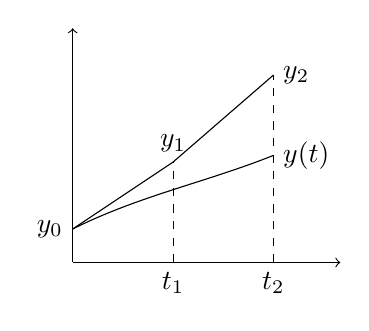
\begin{tikzpicture}[scale=.85]\draw[->](0,0)--(4,0);\draw[->](0,0)--(0,3.5);\draw(0,.5)..controls(1,1)and(2,1.2)..(3,1.6)node[right]{$y(t)$};\draw(0,.5)--(1.5,1.5)--(3,2.8)node[right]{$y_2$};\draw[dashed](1.5,0)node[below]{$t_1$}--(1.5,1.5)(3,0)node[below]{$t_2$}--(3,2.8);\node[left]at(0,.5){$y_0$};\node[above]at(1.5,1.5){$y_1$};\end{tikzpicture}\end{center}
% Pagina originale 48
\pagina{48}
Un altro metodo che coincide con il metodo di Euler esplicito consiste nel dividere in $N$ intervalli
\[t_0<t_1<t_2<\cdots<t_N\equiv T,\quad y'(t_m)=f(t_m,y_m)\simeq\frac{y_{m+1}-y_m}h\quad\text{(differenze in avanti)}.\]
Minore è $h$, più precisa sarà la soluzione. Il metodo è convergente se migliora l'approssimazione diminuendo opportunamente il passo $h$.
\subsection*{Studio della convergenza}
\[e(t_m,h):=y(t_m)-y_m\]
è l'errore globale. La convergenza consiste nell'annullarsi di $e(t_m,h)$ quando $h\to0$. Uno schema è convergente nel punto $T$ quando
\[\lim_{h\to0}e(t_m,h)=0\quad\Longleftrightarrow\quad\lim_{m\to+\infty}y_m=y(T).\]
Supponiamo di aver applicato Euler esplicito e indico con $y_m$ la soluzione approssimata. Chiamo $z(t)$ la soluzione dell'equazione differenziale che si ottiene prendendo $y_m$ come dato iniziale. Nella soluzione globale ci sono due errori:
\begin{enumerate}\item Errore di troncamento locale:
\[I_m(h,f):=z(t_{m+1})-[\underbrace{y_m}_{z(t_m)}+hf(t_m,y_m)].\]
Quest'errore è dovuto alla sostituzione della soluzione con la tangente.\end{enumerate}
% Pagina originale 49
\pagina{49}
\[\tau_m(h,f)=\frac{I_m(h,f)}h=\frac{z(t_m+h)-z(t_m)}h-f(t_m,z(t_m))\]
è chiamato errore di discretizzazione locale. Quando $\tau_m\to0$ per $h\to0$ il metodo è consistente.
\[\lim_{h\to0}\frac{z(t_m+h)-z(t_m)}h=z'(t_m)\Longrightarrow\lim_{h\to0}\tau_m(h,f)=z'(t_m)-f(t_m,z(t_m))=0,\]
perché $f(t_m,z(t_m))=z'(t_m)$. Quindi Euler esplicito è consistente.
Inoltre, espandendo $z(t_m+h)$ con Taylor:
\[z(t_m+h)=z(t_m)+hz'(t_m)+\frac{h^2}2z''(t_m+\theta h),\quad\theta\in(0,1).\]
Osservando $z'(t_m)=f(t_m,y_m)=f(t_m,z(t_m))$ si ha
\begin{align*}I_m(h,f)&=z(t_{m+1})-[y_m+hf(t_m,y_m)]\\&=z(t_m+h)-z(t_m)-hz'(t_m)=\frac{h^2}2z''(t_m+\theta h).\end{align*}
\[\boxed{\tau_m(h,f)=\frac{I_m(h,f)}h=\frac h2z''(t_m+\theta h)},\quad|\tau_m(h,f)|\le Mh,\quad M=\frac12\max_{\theta\in(0,1)}|z''(t_m+\theta h)|.\]
\textit{Nota (pagina 49): l'ultima riga manoscritta riporta $\tau(f,h)=O(h^2)$ e ``metodo di ordine $n$''; la pagina seguente precisa l'ordine corretto $1$.}
% Pagina originale 50
\pagina{50}
In questo caso $\tau(f,h)\propto h$, quindi $\tau=O(h^1)$: il metodo di Euler esplicito è di ordine 1.
\begin{enumerate}\setcounter{enumi}{1}\item Calcolo la tangente passante per il punto $(t_m,y_m)$ e non per $(t_m,y(t_m))$. Questo contributo non è locale in quanto rappresenta l'accumulo di tutti gli errori di troncamento locale commessi in precedenza.\end{enumerate}
Non è garantito che questi errori tendano a zero quando $h\to0$. In sintesi: non è detto che la convergenza a zero degli errori locali porti alla convergenza a zero dell'errore globale.
\[e(x)=0\quad\not\Longleftarrow\quad\tau_m(f,h)\to0\text{ con }h\to0\quad\forall m.\]
Il metodo è stabile se l'accumulo degli errori di troncamento locale si mantiene limitato per $h\to0$.
\[\boxed{\text{Convergenza}\quad\Longleftrightarrow\quad\text{Stabilità}+\text{Consistenza}}.\]
